%Preâmbulo
\documentclass[12pt,a4paper]{article}
\usepackage[brazilian]{babel}
\usepackage[utf8]{inputenc}
\usepackage[left=2cm,right=2cm,top=2cm,bottom=2cm]{geometry}
\usepackage{graphicx}
\usepackage{float}
\graphicspath{{img/}}

\title{Inserir Figura}
\author{César Antônio de Magalhães}
\date{\today}

%Corpo do texto
\begin{document}
	\begin{enumerate}
		\item Calcule o valor de \textrm{x} na Figura \ref{triangulo_retangulo}.
		\begin{figure}[H]
			\centering
			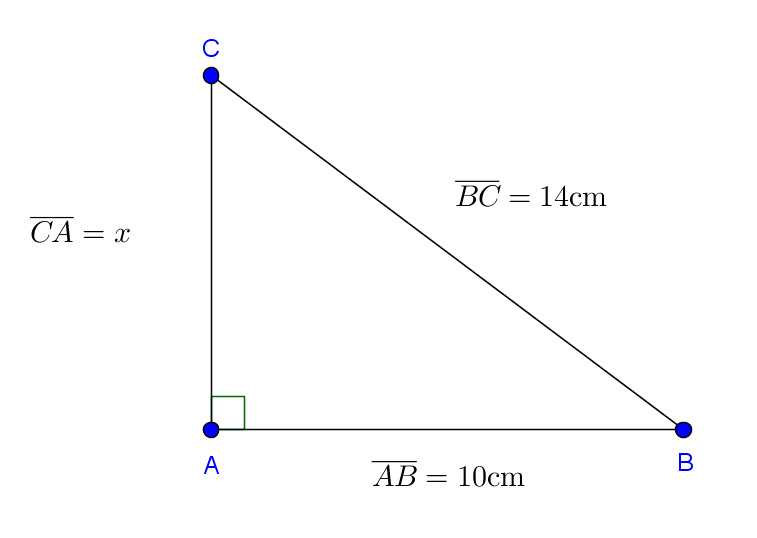
\includegraphics[scale=1]{triangulo_retangulo.png}
			\caption{Questão sobre triângulo}
			\label{triangulo_retangulo}
		\end{figure}
	\end{enumerate}		
\end{document}
